\section{Vista de Distribución}\label{sec:vista-de-distribucion}

En la vista de distribución o \textit{deployment} se plantean escenarios de distribución de los componentes en nodos, con las conexiones entre nodos y los componentes que corre cada uno. Para cada escenario interesa particularmente la descripción de los requerimientos no funcionales que lo justifican \cite{Perovich2003}.

Se utiliza el Diagrama de Deployment UML \cite{Ambysoft2018}. Los nodos físicos llevan el estereotipo \enquote{device}, los servidores y el navegador \enquote{executionEnvironment} y las plataformas en la nube \enquote{PaaS}. Dentro de cada nodo se indican los subsistemas de la Vista Lógica que corre, y cada conexión se rotula con su protocolo.

\begin{figure}[H]
    \centering
    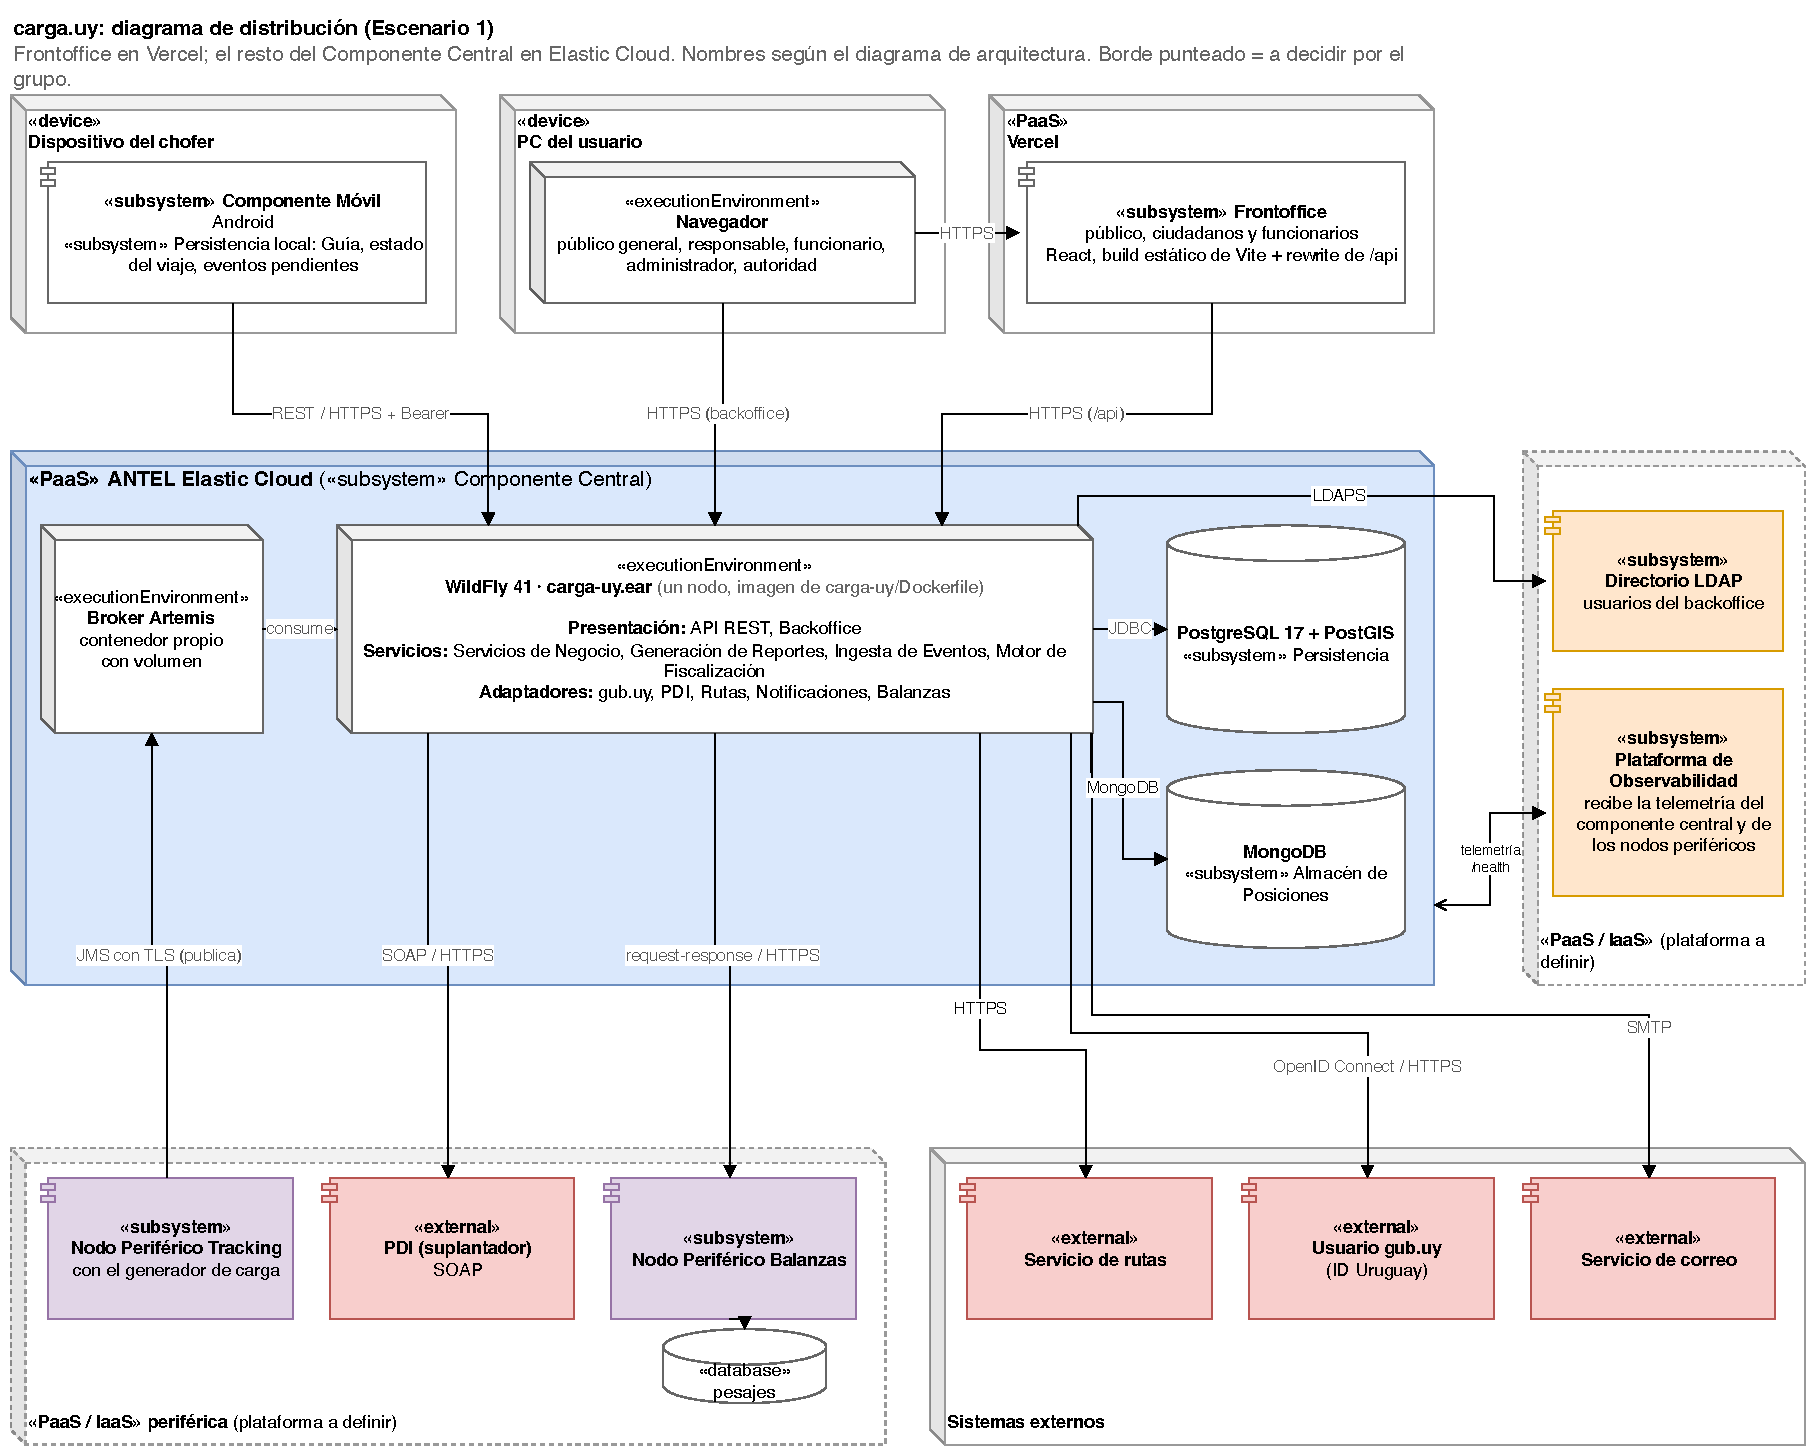
\includegraphics[width=\textwidth]{figures/vista-distribucion.pdf}
    \caption{Vista de Distribución, Escenario 1}
    \label{fig:vista_distrib}
\end{figure}

\subsection{Escenario 1: prototipo}

La Figura \ref{fig:vista_distrib} muestra la distribución prevista para el prototipo. Todas las conexiones entre entornos van por HTTPS (R8), salvo la del nodo de tracking con la mensajería, que se discute al final de esta sección.

\textbf{Dispositivo del chofer.} Corre el Componente Móvil (Android) con su persistencia local, que conserva la Guía, el estado del viaje y los eventos pendientes. Se comunica con el componente central mediante REST sobre HTTPS, con un token \textit{Bearer} (R2).

\textbf{PC del usuario.} El navegador accede al frontoffice y, para el backoffice, directamente al componente central.

\textbf{Vercel.} Sirve el frontoffice, construido en React como sitio estático, y redirige las llamadas a \texttt{/api} hacia el componente central.

\textbf{ANTEL Elastic Cloud (componente central).} Corre el servidor de aplicaciones WildFly con la aplicación empaquetada como EAR (presentación: API REST y backoffice; servicios: Servicios de Negocio, Generación de Reportes, Ingesta de Eventos y Motor de Fiscalización; adaptadores: gub.uy, PDI, notificaciones y balanzas), la base de datos PostgreSQL y la mensajería (R14).

\textbf{PaaS o IaaS periférica.} Corre los nodos periféricos de balanzas y de tracking, y el suplantador de la PDI (R15). El componente central consulta a balanzas en modalidad solicitud--respuesta (R3) y recibe los eventos de tracking a través de la mensajería (R4).

\textbf{Sistemas externos.} Usuario gub.uy (OpenID Connect) y el servicio de correo (SMTP).

\pendiente{describir los requerimientos no funcionales que justifican este escenario.}

\pendiente{confirmar con el tutor que los frontoffices pueden servirse desde Vercel: la letra ubica los frontoffices en el componente central y exige que el componente central corra en Elastic Cloud (R14).}

\pendiente{resolver la ubicación de la mensajería: el diagrama la muestra como un broker aparte, \enquote{a definir}, mientras que el grupo había decidido embeberla en el servidor de aplicaciones (DA02). Definir también cómo cumple R8 la conexión del nodo de tracking con la mensajería, porque los protocolos de los brokers no son HTTPS.}

\pendiente{agregar los componentes de observabilidad (colector de telemetría, trazas y métricas) y, si se adopta, la separación entre el generador de carga y el nodo de tracking.}

\subsection{Escenario 2}

\pendiente{definir si corresponde un segundo escenario, por ejemplo con varias instancias del servidor de aplicaciones detrás de un balanceador para verificar el escalado horizontal (AC07) en la prueba de performance.}
